% --------------------------------------------------------- EXPERIMENTAL DESIGN
\section{Experimental design}
\label{sec:experimental-design}

The experiments were designed to answer the three research questions and guide the development
of the pipeline. Clustering and labeling methods were compared to determine which to use at
each step.

This section also explains why the benchmarks described in Section~\ref{sec:method-benchmarks}
were chosen and how they are used to assess the pipeline. Their known categories provide a
reference for judging how well the discovered groups and the final page labels match known
topics.

\subsection{Clustering}
\label{sec:experiment-comparisons}

The initial comparison tested BERTopic~\cite{grootendorst2022bertopic}, LDA~\cite{blei2003lda},
a local S\textsuperscript{3} baseline~\cite{kardos2025s3}, FASTopic~\cite{wu2024fastopic},
CombinedTM~\cite{bianchi2021combinedtm} and TopicGPT-Lite, a local adaptation of
TopicGPT~\cite{pham2024topicgpt}. The models were tested on separate English and German
samples of the DLR crawl. The comparisons considered word coherence, coverage and cluster
separation (Section~\ref{sec:method-metrics}), alongside the topic counts and keyword lists.

The DLR experiments gave no clear basis for choosing a topic count (Section~\ref{sec:rq1-nok}).
The crawl mixes many subjects with repeated navigation text and page templates
(Section~\ref{sec:method-corpus}). A cluster of pages that share a template can score well on
word coherence because it repeats the same terms. The same models were tested on the GDELT control described
in Section~\ref{sec:method-benchmarks}. Because the articles cover one event, the flood and
the response to it, a small number of topics was expected.

\measured{} The separate silhouette sweep in Figure~\ref{fig:gdelt-silhouette} scored two groups
highest among the tested counts. BERTopic also returned two groups in the corrected GDELT run
(Figure~\ref{fig:gdelt-models}).

\noindent\begin{minipage}{\linewidth}
\centering
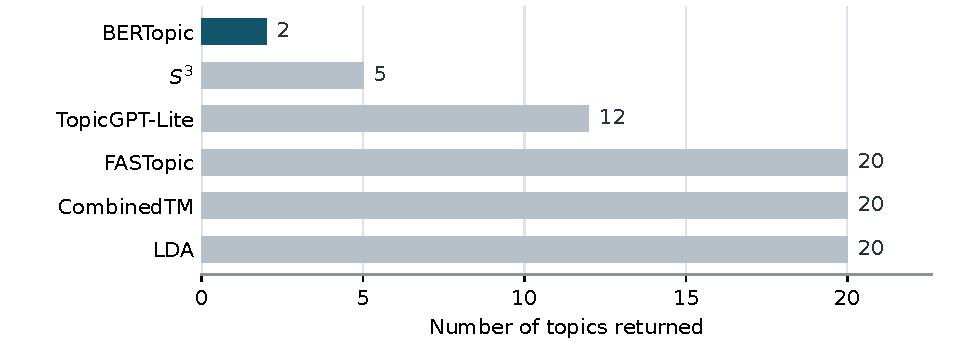
\includegraphics[width=0.93\linewidth]{figs/fig_gdelt_models.pdf}
\captionof{figure}{Topic counts on the GDELT flood corpus. \measured{} The bars show topics
with assigned articles in the corrected run, excluding noise. BERTopic used a minimum cluster
size of 100. S3 returned the lowest count in its search range.
TopicGPT-Lite was asked for 20 topics. FASTopic, CombinedTM and LDA were set to 20.
Source \texttt{output/gdelt\_ahrtal\_v2/}\allowbreak\texttt{eval\_results.json}.}
\label{fig:gdelt-models}
\end{minipage}

The GDELT result supported the choice of BERTopic for the pipeline. Using the E5 vectors,
it returned few groups on the focused control and many fine topics on the DLR crawl
without a preset topic count. Its keywords make the topics easier to inspect
(Section~\ref{sec:method-bertopic}). Another reason for choosing BERTopic was its
\texttt{min\_topic\_size} setting, which controls how small a cluster can be. RQ3 varies this
setting to test how coarse or fine the topics should be, using LDA as a fixed coarse reference
(Section~\ref{sec:rq3-hierarchy}).

\subsection{Document labeling}
\label{sec:experiment-labeling}

The first labeling experiment followed a suggestion from the OpenSearch@DLR~1.0 team to use an
existing labeling model with its own embeddings. Lbl2Vec~\cite{schopf2021lbl2vec} was tested
with BERTopic's keywords. It trained a separate Doc2Vec~\cite{le2014doc2vec} model on each
benchmark and used the keywords to find documents from which to build topic vectors.
Its 300-dimensional Doc2Vec vectors occupied a different embedding space from the
1{,}024-dimensional E5 vectors that BERTopic had clustered.

Once BERTopic had found the clusters, the task was to assign each document to one of them.
This motivated comparing each document with the cluster centroids in the same E5 space
(Section~\ref{sec:method-coverage}). The comparisons run on a CPU using the saved E5 vectors,
which avoids the cost of training and running a second embedding model.

The original BERTopic clusters give the reference score before labeling. \measured{} They had
the highest NMI on each benchmark in Figure~\ref{fig:labeling-benchmarks}. Nearest centroid
stayed closer to that score than Lbl2Vec did. Lbl2Vec changed both the embedding model and
the way topics were represented, so this comparison cannot isolate how much of the loss
came from switching to Doc2Vec.

\noindent\begin{minipage}{\linewidth}
\centering
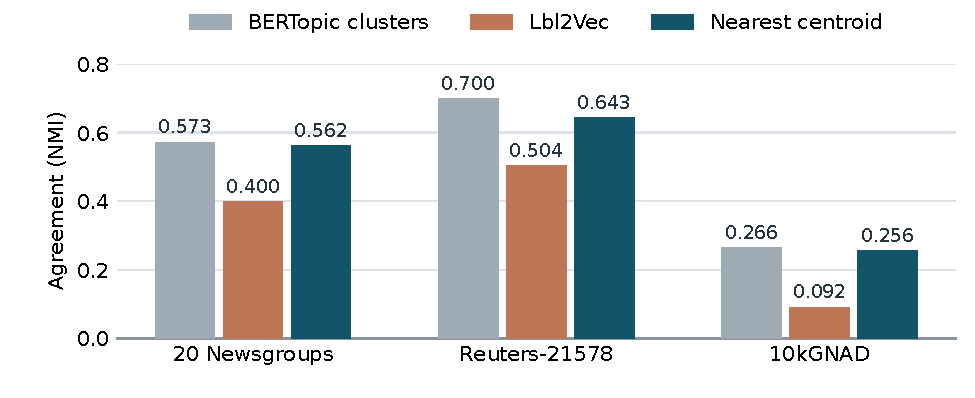
\includegraphics[width=0.98\linewidth]{figs/fig_labeling_benchmarks.pdf}
\captionof{figure}{Agreement with known classes before and after labeling, measured by NMI
(Section~\ref{sec:method-metrics}). \measured{} Within each benchmark all three scores use the
same documents, with BERTopic noise excluded and minimum cluster size fixed at 100.
Sources \texttt{data/groundtruth/} and \texttt{output/groundtruth/}.}
\label{fig:labeling-benchmarks}
\end{minipage}

\measured{} Across the prepared benchmarks, Lbl2Vec returned labels for about 93\% of documents
on each English benchmark and 99.8\% on 10kGNAD. Nearest centroid labeled every document that
reached the labeling step. This covered 99.5\% of 20 Newsgroups and 100\% of the other two
benchmarks. These results led to the choice of nearest centroid for the pipeline.

\subsection{Evaluation measures}
\label{sec:method-metrics}

The evaluation measures were chosen to assess how coherent and distinct the topics are and
how well the clusters are separated. They also show whether every document receives a label
and how closely the assigned labels match the known classes on the benchmarks.

\begin{description}[leftmargin=1.3em,style=nextline,itemsep=3pt]
\item[Word coherence from NPMI.]
Normalised pointwise mutual information (NPMI) scores topic word lists from text
alone~\cite[p.~533]{lau2014tealeaves}. It was chosen so that models could be compared on the
unlabelled DLR crawl using the same reference text.

NPMI checks whether two words appear together more
often than expected from how common each word is on its own~\cite[Eq.~(7)]{bouma2009npmi}.
The reference text is read in short stretches called windows, each up to $h$ tokens long.
For two words $u$ and $v$, $p_h(u)$ and $p_h(v)$ are the shares of windows with each word.
The share of windows with both words is $p_h(u,v)$. The pair score is
\[
  f_h(u,v)=
  \frac{\log\!\bigl((p_h(u,v)+\varepsilon)/(p_h(u)p_h(v))\bigr)}
       {-\log\!\bigl(p_h(u,v)+\varepsilon\bigr)},
\]
where the small number $\varepsilon=10^{-12}$ lets the formula work even when the two words
never appear together.

\emph{Example.} Suppose \emph{ice} and \emph{hockey} each appear in 20 out of 100 windows.
If they appeared independently, both would be expected in $100\times0.20\times0.20=4$ windows.
Suppose they actually appear together in 10. Putting these counts into the formula gives an
NPMI of about $0.40$. The score is positive because the words appear together more often
than expected.

To score a topic, take the average over all pairs of its $m$ top words
$W=(w_1,\ldots,w_m)$. This evaluation uses 10-token windows~\cite[Table~2]{roder2015coherence}.
\[
  \mathrm{NPMI}(W)=\frac{2}{m(m-1)}\sum_{1\le i<j\le m}f_{10}(w_i,w_j).
\]

\item[Word coherence from $C_v$.]
$C_v$ was used as a second check on whether a topic's words fit together. It checks how well
each word fits the pattern of the whole list~\cite[Eqs.~(34)--(35) and Table~2]{roder2015coherence}.

For each word $w$, use the NPMI formula to score it with every word $u$ in the topic list
$W$, including itself. Use 110-token windows. Write the scores as a vector
$v_w=(f_{110}(w,u))_{u\in W}$. Add the word vectors to get $v_W=\sum_{w\in W}v_w$.
Compare each $v_w$ with $v_W$ using cosine similarity and average the results over the
$m$ words. The notation $\|\cdot\|_2$ means vector length.
\[
  C_v(W)=\frac{1}{m}\sum_{w\in W}
  \frac{v_w\cdot v_W}{\|v_w\|_2\,\|v_W\|_2}.
\]

\emph{Example.} Suppose \emph{ice} and \emph{hockey} appear in the same 20 out of 100 windows.
The word \emph{printer} also appears in 20 windows and shares four with the other two words.
In the order \emph{ice}, \emph{hockey}, \emph{printer}, the rounded vectors are
$(1,1,0)$ for both \emph{ice} and \emph{hockey}, and $(0,0,1)$ for \emph{printer}.
Their sum is $(2,2,1)$. Compared with the sum, the first two words score about $0.94$ each,
and \emph{printer} scores about $0.33$. The average gives $C_v\approx0.74$.

Both coherence measures use up to ten words per topic. The evaluation drops words outside
its reference vocabulary and skips topics left with fewer than two words. Each model's
score is the mean across the remaining topics, with higher values indicating stronger
coherence (\texttt{scripts/run\_eval.py}).

\item[Topic diversity.]
Topics can score well on coherence and still use many of the same words. Topic diversity
was chosen to check for this repetition across topics.

Make one list $L$ with up to ten top words from each topic
(\texttt{scripts/}\allowbreak\texttt{eval\_junk\_filtered.py}). Divide the number of different
words in $L$ by $|L|$, the number of entries including repeats~\cite[p.~448]{dieng2020etm}.
\[
  \mathrm{Diversity}=\frac{|\{w:w\in L\}|}{|L|}.
\]
A higher value means less repetition between topic descriptions.

\emph{Example.} Suppose one topic lists \emph{ice}, \emph{hockey} and \emph{skates}.
Another lists \emph{ice}, \emph{snow} and \emph{winter}. There are six entries and five
different words because \emph{ice} appears twice. The diversity is $5/6\approx0.83$.

\item[Coverage.]
Let $N_{\mathrm{input}}$ be the number of input documents and $N_{\mathrm{labelled}}$ the
number that receive a topic. Coverage checks the requirement in
Section~\ref{sec:intro-neutrality}.
\[
  \mathrm{Coverage}(\%)=100\,\frac{N_{\mathrm{labelled}}}{N_{\mathrm{input}}}.
\]

\item[Silhouette.]
For document $i$, let $a_i$ be the mean cosine distance to the other documents in its
cluster. Let $b_i$ be the smallest mean distance to the documents of any other cluster.
The overall score averages the individual scores over the $n$ evaluated documents
\cite[pp.~55--56,~59]{rousseeuw1987silhouette}.
\[
  s_i=\frac{b_i-a_i}{\max(a_i,b_i)},\qquad
  \mathrm{Silhouette}=\frac{1}{n}\sum_{i=1}^{n}s_i.
\]
A document alone in its cluster contributes zero. Higher values indicate better separation.

\item[Davies--Bouldin index.]
Let $K$ be the number of evaluated clusters, $\mu_k$ the mean vector of cluster $k$, and
$S_k$ the mean Euclidean distance of its document vectors to $\mu_k$. The denominator
$\|\mu_k-\mu_\ell\|_2$ is the Euclidean distance between the two cluster centres.
For each cluster $k$, the index takes the worst ratio of spread to separation over the
other clusters $\ell$ and then averages these ratios~\cite[p.~225]{davies1979cluster}.
\[
  \mathrm{DB}=\frac{1}{K}\sum_{k=1}^{K}
  \max_{\ell\ne k}\frac{S_k+S_\ell}{\|\mu_k-\mu_\ell\|_2}.
\]
Lower values indicate better separation. The model comparison computes both geometry
scores on sampled documents in the shared UMAP evaluation space
(\texttt{scripts/run\_eval.py}).

\item[Agreement with reference labels.]
Let $\Omega$ be the assignment to clusters $\omega_1,\ldots,\omega_K$, and let $C$ be
the reference classification into classes $c_1,\ldots,c_J$ on the same $N$ scored
documents. Write $p_k=|\omega_k|/N$ and $q_j=|c_j|/N$ for the cluster and class shares.
Write $p_{kj}=|\omega_k\cap c_j|/N$ for the share in both. The entropies $H(\Omega)$
and $H(C)$ measure uncertainty in cluster and class membership, and mutual information
$I$ measures how much they tell us about each other.
\[
\begin{aligned}
  H(\Omega)&=-\sum_{k=1}^{K}p_k\log p_k,&
  H(C)&=-\sum_{j=1}^{J}q_j\log q_j,\\
  I&=\sum_{k=1}^{K}\sum_{j=1}^{J}p_{kj}\log\frac{p_{kj}}{p_kq_j}. &&
\end{aligned}
\]
Terms with $p_{kj}=0$ contribute zero to $I$. Normalised mutual information (NMI)
divides $I$ by the mean of the two entropies. Adjusted mutual information (AMI) also
subtracts the expected mutual information $E[I]$ under random assignments with the
same cluster and class sizes~\cite[Table~2, p.~2841 and Sec.~4.1]{vinh2010information}.
\[
  \mathrm{NMI}=\frac{I}{\tfrac12[H(\Omega)+H(C)]},\qquad
  \mathrm{AMI}=\frac{I-E[I]}{\tfrac12[H(\Omega)+H(C)]-E[I]}.
\]
Purity counts the documents in the most common reference class of each cluster and
divides by $N$~\cite[Eq.~(16.1), p.~357]{manning2008ir}.
\begin{equation}
  \mathrm{Purity}=\frac{1}{N}\sum_{k=1}^{K}\max_{1\le j\le J}|\omega_k\cap c_j|.
  \label{eq:benchmark-purity}
\end{equation}
Higher values indicate greater agreement. All three scores are calculated only on
labelled benchmarks (\texttt{scripts/run\_groundtruth\_metrics.py}).

\item[Elapsed time.]
For a timed operation, $t_{\mathrm{start}}$ and $t_{\mathrm{end}}$ are the clock
readings immediately before and after it. This measure is used for the exploratory
search experiments in Section~\ref{sec:setaside-speed}.
\[
  t_{\mathrm{elapsed}}=t_{\mathrm{end}}-t_{\mathrm{start}}.
\]
\end{description}

Ground-truth scores use the documents available in both a run's output and the prepared
reference labels. Raw BERTopic scores exclude the noise label $-1$. Different runs can
therefore be scored on different document sets; coverage must be read alongside agreement
scores. The largest-class baseline for purity must also be calculated on the set actually
scored.

The language-model judge used in earlier exploration is excluded from this evaluation panel.

\subsection{The purity floor}
\label{sec:experimental-purity-floor} \proved{} Purity can never
fall below the share of the largest class, provided every document carries exactly one class and is
placed in exactly one cluster. Figure~\ref{fig:purityfloor} shows the argument on a ten-document example.
Use the purity definition in Equation~\eqref{eq:benchmark-purity} and let $c^\ast$ be
the largest reference class.
\begin{enumerate}[leftmargin=1.5em,itemsep=2pt]
\item \emph{Inside one cluster.} The largest class count inside a cluster must be at least the
count belonging to $c^\ast$:
\[
  \max_j |\omega_k \cap c_j| \;\ge\; |\omega_k \cap c^\ast| \qquad \text{for every } k.
\]
\item \emph{Adding over clusters.} Add this inequality over all clusters and divide by $N > 0$:
\[
  \text{purity} \;\ge\; \frac{1}{N}\sum_{k=1}^{K} |\omega_k \cap c^\ast|.
\]
\item \emph{Counting the largest class.} Each document in $c^\ast$ belongs to exactly one
cluster, so these counts add up to $|c^\ast|$:
\[
  \sum_{k=1}^{K} |\omega_k \cap c^\ast| \;=\; |c^\ast|.
\]
\end{enumerate}
Together, $\text{purity} \ge |c^\ast|/N$. Putting every document in one cluster reaches this bound
exactly, so it cannot be raised. Any clustering that places every document therefore scores at
least $0.4887$ on Reuters, but only $0.0544$ on 20 Newsgroups (Section~\ref{sec:neutrality}).

\begin{figure}[t]\centering
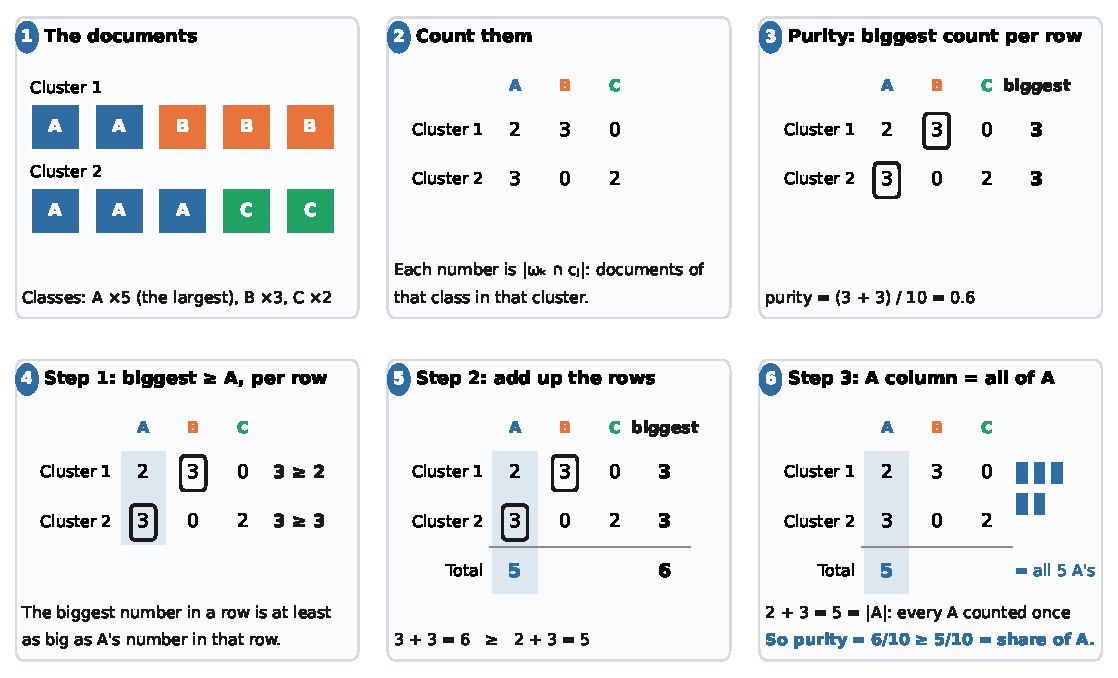
\includegraphics[width=\textwidth]{figs/fig_purity_floor}
\caption{Visual proof of the purity floor, one step per panel, on ten documents with classes A
(5 documents, the largest), B (3) and C (2). \textbf{(1)}~The documents in two clusters.
\textbf{(2)}~The same clustering as counts, one row per cluster. \textbf{(3)}~Purity adds the
biggest count in each row (boxed). \textbf{(4)--(6)}~The three steps of the proof: in each row the
boxed count is at least A's count (shaded); adding up the rows keeps the inequality; and the A
column adds up to all of A.}
\label{fig:purityfloor}
\end{figure}

